\section{Results}\label{sec:results}

All numbers in this section are for the S\&P~500 with gpt-oss-20b, prompt A, $N=20$, evaluated over the 26 rebalancing decisions of 2025. \pending{Other markets and models will be added as columns or panels of the same tables.}

\subsection{What the views contain}\label{sec:res_q}
Table~\ref{tab:q} describes $\bq$ before it enters the portfolio. The cross-sectional ranking of $q_i$ is almost the ranking of the trailing ten-day return (rank correlation 0.96). Its rank correlation with the next two-week return is 0.02, and the slope of the next return on $q_i$ is slightly negative. Given only recent returns, the model extrapolates them. At the two-week horizon in 2025 that signal had no predictive value; the trailing ten-day mean itself had a rank correlation of 0.01 with the next period. The views are also uniformly optimistic: the average $q_i$ is 0.20\% per day (about 65\% annualized), against a realized average of 0.08\%.

\begin{table}[t]
\centering
\caption{What the LLM views contain. Rank correlations are cross-sectional Spearman correlations computed at each rebalancing date and averaged over the 34 dates. US, gpt-oss-20b, prompt A, $N=20$.}
\label{tab:q}
\small
\begin{tabular}{lr}
\toprule
Quantity & Value \\
\midrule
Rank correlation of $q_i$ with the trailing 10-day mean return & 0.959 \\
Rank correlation of $q_i$ with the next two-week mean return & 0.017 \\
Rank correlation of the trailing 10-day mean with the next two-week mean & 0.012 \\
Slope of the next two-week return on $q_i$ (both demeaned by date) & -0.048 \\
Mean $q_i$ (\% per day) & 0.200 \\
Mean realized return (\% per day) & 0.080 \\
\bottomrule
\end{tabular}

\end{table}

\subsection{Test (a): is dispersion informative about view error?}\label{sec:res_a}
Table~\ref{tab:calib} reports the shape and level diagnostics of Section~\ref{sec:criteria}. The raw rank correlation between $s_i^2$ and the squared error is 0.19. Part of it is volatility: dispersion and the trailing variance have a rank correlation of 0.33. After standardizing both by $\hat\sigma_i^2$, the correlation is 0.15; the partial rank correlation given $\hat\sigma_i^2$ is 0.12; computed within each date it averages 0.12, is positive on 79\% of dates and has a $t$-statistic of 4.4 across dates. Test (a) is passed: LLM dispersion carries information about forecast error that volatility does not.

The level diagnostics follow Eq.~\eqref{eq:decomp}. An interval built from $s_i^2$ alone covers the realized return 36\% of the time at the nominal 95\% level. Adding the return-noise variance gives 92.8\%, close to nominal, and the noise variance by itself already gives 91.3\%. On average $s_i^2$ is about one ninth of $\hat\sigma_i^2/h$. Most of the forecast error is return noise that no forecaster could remove, and the ``overconfidence'' of the raw interval is mostly the omitted noise term.

All diagnostics are nearly identical for $N=5$, 10 and 20. The information in dispersion saturates by $N=5$--10, so the number of queries per stock can be cut by half or more without loss.

\begin{table}[t]
\centering
\caption{Dispersion as an uncertainty signal. $e^2=(q_i-\bar r_i)^2$, $\hat\sigma^2$ the trailing 126-day variance, $h$ the number of trading days in the holding period. $N=5$ and $10$ are averages over three random subsets of the 20 draws. Coverage is the share of pairs with $|q_i-\bar r_i| \le 1.96\times$ the stated standard deviation. 1{,}700 pairs over 34 dates.}
\label{tab:calib}
\small
\begin{tabular}{lrrr}
\toprule
 & $N=5$ & $N=10$ & $N=20$ \\
\midrule
$\rho(s^2, e^2)$ & 0.172 & 0.173 & 0.187 \\
$\rho(s^2/\hat\sigma^2, e^2/\hat\sigma^2)$ & 0.148 & 0.141 & 0.150 \\
Partial $\rho$ given $\hat\sigma^2$ & 0.123 & 0.116 & 0.124 \\
Within-date mean & 0.117 & 0.110 & 0.123 \\
Share of dates $>0$ & 0.745 & 0.775 & 0.794 \\
$t$ (across dates) & 4.102 & 4.220 & 4.417 \\
\midrule
95\% cov., $s^2$ & 0.314 & 0.344 & 0.362 \\
95\% cov., $s^2+\hat\sigma^2/h$ & 0.923 & 0.927 & 0.928 \\
95\% cov., $\hat\sigma^2/h$ & 0.909 & 0.912 & 0.913 \\
\bottomrule
\end{tabular}

\end{table}

\subsection{Test (b): does the dispersion improve the portfolio?}\label{sec:res_b}
Table~\ref{tab:omega} and Figure~\ref{fig:omega} hold $\bq$ fixed and vary only $\Om$. Test (b) fails in every specification. The empirical $\Om$ has the lowest Sharpe ratio of all variants in three of the four specifications. It is below the constant $\Om$ by 0.49 to 0.97, significant at 5\% in all four. It is below He--Litterman by 0.51 to 1.15, significant in three of four. Level matching and the 10\% cap raise the Sharpe ratio of every variant except the shuffled one, whose raw value (0.48, from a single random permutation) is the outlier of the table; He--Litterman is unaffected by level matching by construction. Neither changes the conclusion of test (b).

Recalibration removes part of the damage: the linear-calibrated $\Om$ is better than the empirical $\Om$ in all four specifications and the isotonic one in three. Neither beats the conventions. The linear-calibrated $\Om$ is below the constant $\Om$ in all four specifications ($p<0.05$) and significantly below He--Litterman in three. Assigning the same dispersion values to randomly chosen stocks (shuffled) gives a higher Sharpe ratio than assigning them to the right stocks in all four specifications; the difference is significant in the raw specification ($p<0.01$) and marginal under level matching ($p=0.06$).

\begin{table}[t]
\centering
\caption{Annualized Sharpe ratio of Black--Litterman portfolios that share the LLM views $\bq$ and differ only in $\Om$, under four specifications (Section~\ref{sec:omega_variants}). He--Litterman is already at the He--Litterman level, so its level-matched entries equal the unmatched ones. Lower panel: Sharpe ratio differences, paired circular block bootstrap; $^{*}$, $^{**}$, $^{***}$: two-sided $p<0.10, 0.05, 0.01$. 2025, 10 bp costs, $\tau$ chosen out of sample.}
\label{tab:omega}
\small
\begin{tabular}{lrrrr}
\toprule
$\bm{\Omega}$ & Raw & Level-matched & 10\% cap & Level-matched + cap \\
\midrule
Empirical ($s_i^2$) & -2.02 & -1.46 & -0.28 & -0.34 \\
Constant & -1.32 & -0.49 & 0.31 & 0.15 \\
Shuffled & 0.48 & -0.50 & -0.12 & -0.07 \\
He--Litterman ($\tau\Sigma_{ii}$) & -0.87 & -0.87 & 0.23 & 0.23 \\
Isotonic-calibrated & -1.45 & -0.92 & -0.30 & -0.09 \\
Linear-calibrated & -1.81 & -1.00 & -0.25 & -0.07 \\
\midrule
Empirical $-$ Constant & -0.70$^{**}$ & -0.97$^{**}$ & -0.59$^{**}$ & -0.49$^{**}$ \\
Linear-calibrated $-$ Constant & -0.49$^{**}$ & -0.52$^{**}$ & -0.56$^{***}$ & -0.22$^{**}$ \\
Empirical $-$ He--Litterman & -1.15$^{***}$ & -0.58 & -0.51$^{**}$ & -0.57$^{***}$ \\
Linear-calibrated $-$ He--Litterman & -0.94$^{***}$ & -0.13 & -0.48$^{***}$ & -0.30$^{**}$ \\
\bottomrule
\end{tabular}

\end{table}

\begin{figure}[t]
\centering
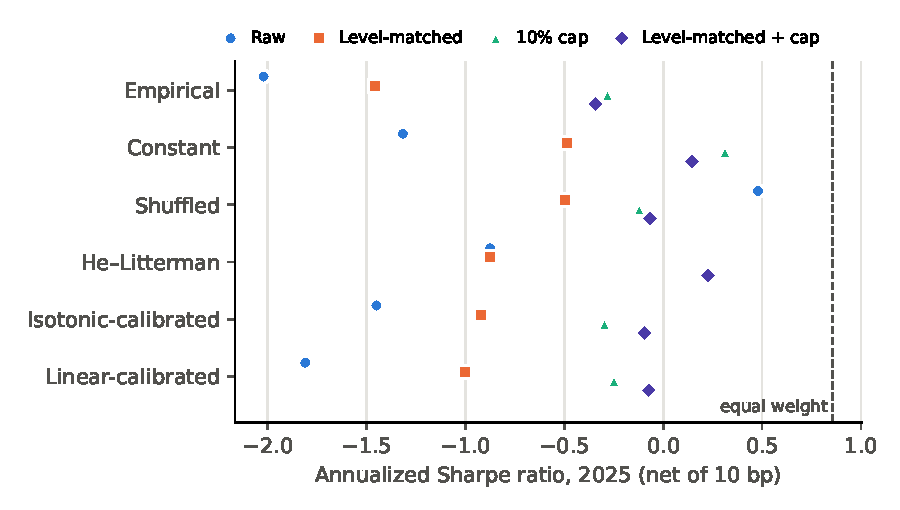
\includegraphics[width=0.85\linewidth]{figures/fig_omega}
\caption{Sharpe ratio of each $\Om$ variant under the four specifications; same data as Table~\ref{tab:omega}. The dashed line is the equal-weight portfolio.}
\label{fig:omega}
\end{figure}

\subsection{Why informative dispersion has negative decision value}\label{sec:res_why}
Tests (a) and (b) disagree. Figure~\ref{fig:deciles} shows why. It sorts stocks into deciles of $s_i^2$ within each date and plots the average dispersion, squared error and return noise per decile. From the lowest to the highest decile, $s_i^2$ rises by a factor of 121. The realized squared error rises by a factor of 4.0, and the return noise, which is pure volatility, by 3.2. Within a single date the 90th percentile of $s_i^2$ is 22 times the 10th percentile; for the trailing variance the ratio is 5.6.

\begin{figure}[t]
\centering
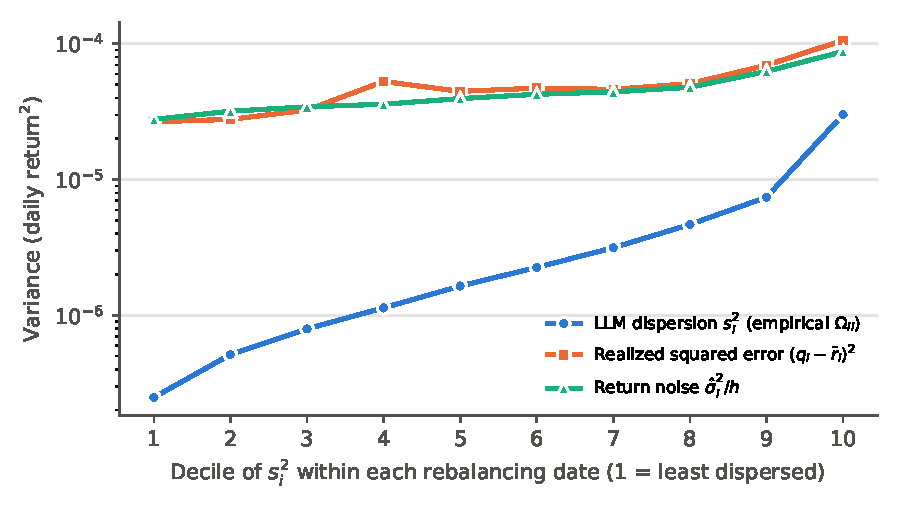
\includegraphics[width=0.85\linewidth]{figures/fig_deciles}
\caption{Dispersion overstates differences in forecast error. Stocks are sorted into deciles of $s_i^2$ within each rebalancing date; lines show decile averages (log scale). The realized squared error tracks the return noise; the dispersion spans two orders of magnitude more.}
\label{fig:deciles}
\end{figure}

The ordering in $s_i^2$ is right on average, but its magnitude is not. Used as $\Om$, the empirical mapping trusts the least dispersed views about a hundred times more than the most dispersed ones, while their actual errors differ by a factor of about four, most of which volatility, and hence He--Litterman, already captures. Because $\bq$ carries no predictive information (Section~\ref{sec:res_q}), concentrating weight on a subset of views only adds variance: the uncapped empirical portfolio puts up to 91\% in one stock. A constant $\Om$ spreads the same views evenly and loses less.

Two features of the draws help explain the exaggerated spread. First, dispersion follows the size of the recent move: the rank correlation between $s_i^2/\hat\sigma_i^2$ and $|$trailing ten-day return$|/\hat\sigma_i$ is 0.52. The model disagrees with itself more when it has a large move to extrapolate, which is also when the extrapolated view is far from a realized return near zero. Second, answers are discrete: the 20 draws for a stock-date contain on average 10 distinct values, the most common value accounts for 29\% of them, and 0.05\% per day alone accounts for 10\% of all 34{,}762 answers. Low dispersion often means the model repeated a round number, not that it was more certain.

We also tested whether the common optimism of $\bq$ drives the result, by shifting all views so that their cross-sectional mean equals that of the prior $\bm{\Pi}$. This leaves the empirical portfolio unchanged ($-2.01$ against $-2.02$; Table~\ref{tab:center} in the appendix). The harm comes from the cross-sectional shape of $\Om$, not from the level of $\bq$.

\subsection{Reference portfolios}\label{sec:res_ref}
Table~\ref{tab:reference} places these results among portfolios without LLM views. Equal weight has a Sharpe ratio of 0.86 and no Black--Litterman portfolio with LLM views comes close; the best is the constant $\Om$ with a 10\% cap (0.31). Black--Litterman with a momentum view behaves like the LLM version ($-1.65$ uncapped), as expected from Table~\ref{tab:q}. The top-ten portfolio by LLM $q_i$ (0.73) and the top-ten momentum portfolio (0.71) are statistically indistinguishable (difference 0.02, $p=0.92$). The original study's finding that LLM views in Black--Litterman beat equal weight does not hold with point-in-time data, a documented-cutoff model and an out-of-sample $\tau$.

\begin{table}[t]
\centering
\caption{Reference portfolios, 2025, 10 bp costs. Max $w$: largest single weight at any rebalancing date. Right block: same strategy with a 10\% weight cap, where it applies.}
\label{tab:reference}
\small
\begin{tabular}{lrrrrr|rr}
\toprule
 & Sharpe & CAGR & Vol. & MDD & Max $w$ & \multicolumn{2}{c}{10\% cap} \\
 & & & & & & Sharpe & MDD \\
\midrule
Equal weight & 0.86 & 0.19 & 0.17 & -0.18 & 0.02 & -- & -- \\
Market-cap weight & 0.79 & 0.21 & 0.21 & -0.21 & 0.13 & -- & -- \\
MVO, 126-day mean & 0.54 & 0.15 & 0.23 & -0.19 & 0.44 & 0.38 & -0.19 \\
BL prior only (no views) & -0.12 & 0.01 & 0.14 & -0.13 & 0.27 & 0.03 & -0.13 \\
BL, 126-day mean view & 0.51 & 0.14 & 0.23 & -0.19 & 0.44 & 0.33 & -0.18 \\
BL, momentum view & -1.65 & -0.36 & 0.27 & -0.44 & 0.86 & 0.05 & -0.14 \\
Top-10 momentum & 0.71 & 0.18 & 0.21 & -0.19 & 0.10 & -- & -- \\
MVO on LLM $q$ & -0.82 & -0.18 & 0.25 & -0.34 & 0.91 & 0.35 & -0.17 \\
Top-10 by LLM $q$ & 0.73 & 0.18 & 0.20 & -0.19 & 0.10 & -- & -- \\
BL, LLM $q$, empirical $\Omega$ & -2.02 & -0.36 & 0.23 & -0.38 & 0.91 & -0.28 & -0.14 \\
BL, LLM $q$, He--Litterman $\Omega$ & -0.87 & -0.17 & 0.23 & -0.30 & 0.65 & 0.23 & -0.15 \\
\bottomrule
\end{tabular}

\end{table}

\subsection{Robustness}\label{sec:robust}
\paragraph{Risk aversion $\delta$.} Table~\ref{tab:delta} in the appendix varies $\delta$ over 1.5, 2.5 and 3.5 and a trailing 252-day estimate $\hat\delta = \mathbb{E}[r_m - r_f]/\mathrm{Var}(r_m)$. The estimate ranges from 3.3 to 18.0 (median 5.6) and is never negative in this window. Sharpe ratios of the Black--Litterman portfolios with views change by at most 0.04, and the ordering of $\Om$ variants and all test conclusions are the same for every $\delta$. $\delta$ only scales $\bm{\Pi}$, and the out-of-sample $\tau$ re-balances prior against views. The prior-only portfolio, which has no views to rebalance against, moves more ($-0.26$ to $-0.04$).

\paragraph{Transaction costs.} From 0 to 25 basis points the ordering of the $\Om$ variants does not change (Table~\ref{tab:costs}).

\paragraph{Choice of $\tau$.} The out-of-sample $\tau$ is unstable: for the raw empirical $\Om$ it moves from 10 in the first quarter to $10^{-3}$ in the last, because early choices rest on four months of data. The 10\% cap is our main safeguard against the resulting concentration. \todo{fixed-split robustness (choose $\tau$ once on Sep--Dec 2024).}

\paragraph{Fixed universe.} \todo{Rerun with the universe fixed at 30 August 2024 to quantify the effect of the point-in-time universe alone.}
